\documentclass{article}
\usepackage{enumerate}
\usepackage{graphicx}
\usepackage{subcaption}
\usepackage{hyperref}
\usepackage{epstopdf}
\usepackage{amsmath}
\usepackage{geometry}
\usepackage{color}
\usepackage{makecell}
\geometry{left=2.5cm,right=2.5cm,top=1.5cm,bottom=2cm}

\bibliographystyle{ieeetr}

\title{Generating Criteria}
\author{Jicheng Lu}
\date{}

\begin{document}
\maketitle
%\tableofcontents

\section{Introduction}
\paragraph{}
In this report, we will discuss a general idea of generating criteria of clinical trials for Alzheimer's disease. We first introduce the idea that divides the criteria into two patterns: computable patterns and non-computable patterns. Then we focus on the  computable patterns and  start to build a simple model. Several samples are generated at the end of this report.  \\

\section{General Idea}
\paragraph{}
According to the criteria from the clinical trials, we can observe that the items can be generally divided into two patterns, computable patterns and non-computable patterns. The computable patterns usually contains attributes that can be evaluated with numbers, such as age, years of education or work history, MMSE, modified Hachinski score, etc. Note that some computable attributes can be expressed with time duration. For example, history of active peptic ulcer disease within 1 year of screening. As for the non-computable patterns, the attributes are usually cannot be evaluated with numbers, such as patients willingness, speaking ability, etc. At this stage, we focus on the computable patterns. \\
\\
Among the computable patterns, we can separate them into two types. To the first type, the numbers in the sentence are directly related to the attributes, such as minimum age is 50, MMSE is at least 24, etc. The second type is related with temporal patterns where there are time units in the sentence. For example, use of cholinesterase inhibitors within 2 months of screening. Thus, we will model these two types respectively. In the next section, we introduce a simple model to deal with these two types of computable patterns. \\


\section{A Simple Model}
\paragraph{}
The method of building the simple model is using regular expression. For each pattern, we can define several sentence templates and fill in the corresponding attribute and number. For example, "(attribute) at least (number)", "(attribute) between (number) and (number)", "(Event X) within (t time units) before/after (event Y)". \\
\\
For the patterns where the attribute is directly with the numbers, we define the following templates:
\begin{itemize}
  \item (attribute) at least (number).
  \item (attribute) less than (number).
  \item (attribute) between (number) and (number).
  \item minimum (attribute) (number), maximum (attribute) (number).
\end{itemize}

\noindent For the temporal patterns, we define the following templates:
\begin{itemize}
  \item (event X) within/at least/less than (t time units).
  \item (event X) within/at least/less than (t time units) before/after (event Y).
  \item (cumulative duration t time units) of (event X).
\end{itemize}


\section{Generated Samples}
\paragraph{}
In this section, we present the sample data generated using the simple model. 

\begin{figure}[!hbt]
\centering
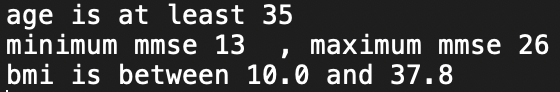
\includegraphics[width=7cm, height=1cm]{figs/sample1.png}
\caption{}
\label{f:res1}
\end{figure}


\begin{figure}[!hbt]
\centering
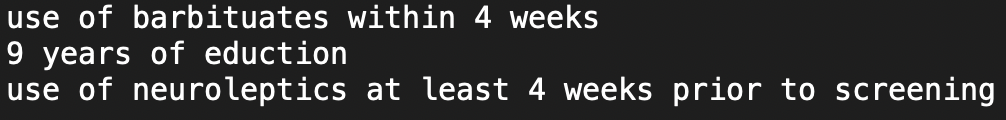
\includegraphics[width=9cm, height=1.5cm]{figs/sample2.png}
\caption{}
\label{f:res2}
\end{figure}

\end{document}












